%include header with all settings
\documentclass[
a4paper,							% alle weiteren Papierformat einstellbar
%landscape,						% Querformat
12pt,						  		% Schriftgrˆfle (12pt, 11pt (Standard))
BCOR1cm,							% Bindekorrektur, bspw. 1 cm
DIV=calc,							% f¸hrt die Satzspiegelberechnung neu aus scrguide 2.4
twoside, 						% zweiseitig twoside/ einseitig oneside
%twocolumn,						% zweispaltiger Satz
%openany,							% Kapitel kˆnnen auch auf linken Seiten beginnen
openright,						% Kapitel beginnen auf der rechten Seite
parskip=half*,			   	% Absatzformatierung s. scrguide 3.1
headsepline,					% Trennline zum Seitenkopf	
footsepline,					% Trennline zum Seitenfufl
%notitlepage,					% in-page-Titel, keine eigene Titelseite
chapterprefix,				% vor Kapitel¸berschrift wird "Kapitel Nummer" gesetzt
appendixprefix,				% Anhang wird "Anhang" vor die ‹berschrift gesetzt 
%normalheadings,			% ‹berschriften etwas kleiner (smallheadings)
%smallheadings, 
%idxtotoc,						% Index im Inhaltsverzeichnis
%liststotoc,					% Abb.- und Tab.verzeichnis im Inhalt
%bibtotoc,					% Literaturverzeichnis im Inhalt
%leqno,						% Nummerierung von Gleichungen links
%fleqn,						% Ausgabe von Gleichungen linksb¸ndig
%draft,						% ¸berlangen Zeilen in Ausgabe gekennzeichnet
%pointlessnumbers,
%DIV13,                % Seitenrand ist 1/13 (Standard: 1/10 -> ziemlich breit)
%BCOR5mm								% Bindekorrektur, links 5mm mehr Platz f¸r Bindung
] {scrreprt}

% breitere seite
\usepackage{a4wide}

%% Normales LaTeX oder pdfLaTeX? %%%%%%%%%%%%%%%%%%%%%%%%%%%%
%% ==> Das neue if-Kommando "\ifpdf" wird an einigen wenigen
%% ==> Stellen benˆtigt, um die Kompatibilit‰t zwischen
%% ==> LaTeX und pdfLaTeX herzustellen.
\newif\ifpdf
\ifx\pdfoutput\undefined
	\pdffalse              %%normales LaTeX wird ausgef¸hrt
\else
	\pdfoutput=1           
	\pdftrue               %%pdfLaTeX wird ausgef¸hrt
\fi


%% Fonts f¸r pdfLaTeX %%%%%%%%%%%%%%%%%%%%%%%%%%%%%%%%%%%%%%%
%% ==> Nur notwendig, falls keine cm-super-Fonts installiert
%\ifpdf
	%\DeclareGraphicsExtensions{.pdf,.jpg,.png}
	%\usepackage{ae}       %%Benutzen Sie nur eines dieser Pakete:
	%\usepackage{zefonts}  %%je nachdem, welches Sie besitzen.
%\else
	%\DeclareGraphicsExtensions{.eps}
	%%Normales LaTeX - keine speziellen Fontpackages notwendig
%\fi

%% Deutsche Anpassungen %%%%%%%%%%%%%%%%%%%%%%%%%%%%%%%%%%%%%
\usepackage[ngerman]{babel}
\usepackage[T1]{fontenc}
%\usepackage[latin1]{inputenc}
\usepackage[utf8]{inputenc}


%% Packages f¸r Grafiken & Abbildungen %%%%%%%%%%%%%%%%%%%%%%
\ifpdf %%Einbindung von Grafiken mittels \includegraphics{datei}
	\usepackage[pdftex]{graphicx} %%Grafiken in pdfLaTeX
\else
	\usepackage[dvips]{graphicx} %%Grafiken und normales LaTeX
\fi
%\usepackage[hang,tight,raggedright]{subfigure} %%Teilabbildungen in einer Abbildung
%\usepackage{pst-all} %%PSTricks - nicht verwendbar mit pdfLaTeX
\let\ifpdf\relax

%% Packages f¸r Formeln %%%%%%%%%%%%%%%%%%%%%%%%%%%%%%%%%%%%%
\usepackage{amsmath}
\usepackage{amsthm}
\usepackage{amsfonts}

\usepackage{times}    % Schriftstil Times New Roman (wie Word)
%\usepackage{url}      % zur Dartellung von URLs mit Befehl \url{}
%\usepackage{xspace}   % Intelligenter Platzhalter nach Makros
\usepackage{booktabs} % schˆne Tabellen mit \toprule, \midrule und \bottomrule

%\usepackage{type1cm} % scalable Fonts
%\usepackage{courier} % Adobe Courier
%\usepackage{sectsty} % eigene Kapitel-Stile
% Control the fonts and formatting used in the table of contents.
%\usepackage[titles]{tocloft}

%\usepackage[Lenny]{fncychap} % Kapitel-Rahmen am Beginn jedes neuen Kapitels

%% Aesthetic spacing redefines that look nicer to me than the defaults.
%\setlength{\cftbeforechapskip}{2ex}
%\setlength{\cftbeforesecskip}{0.5ex}

%\newcommand{\autor}[1]{\textsc{#1}} % Makro f¸r Autor(en) im Fliefltext
%\newcommand{\degr}{\ensuremath{^\circ}} % Grad-Kreis
%\newcommand{\mum}{\ensuremath{\,\mu\textrm{m}}}
%\newcommand{\subcaption}[1]{\footnotesize\itshape #1}
%\newcommand{\matlab}{\emph{MATLAB}\xspace}

%% Use Helvetica-Narrow Bold for Chapter entries
%\renewcommand{\cftchapfont}{%
 % \fontsize{11}{13}\usefont{OT1}{phv}{bc}{n}\selectfont
%}

% \renewcommand{\baselinestretch}{1.5} % Zeilenabstand 1.5

% Verhindern von "`Schusterjungen"' und "`Hurenkindern"'
\clubpenalty = 10000
\widowpenalty = 10000
\displaywidowpenalty = 10000
\tolerance=500 %Zeilenumbruch


%% Zeilenabstand %%%%%%%%%%%%%%%%%%%%%%%%%%%%%%%%%%%%%%%%%%%%
\usepackage{setspace}
%\singlespacing        %% 1-zeilig (Standard)
\onehalfspacing       %% 1,5-zeilig
%\doublespacing        %% 2-zeilig
\usepackage{fancyhdr} %%Fancy Kopf- und Fuflzeilen
\usepackage{longtable} %%F¸r Tabellen, die eine Seite ¸berschreiten
\usepackage[babel,german=guillemets]{csquotes} % Franzˆsische Anf¸hrungszeichen  \enquote{}
% fuer Zitate
%\usepackage[round]{natbib}
\usepackage[numbers,round]{natbib}

% for listings
\usepackage{listings}

%\usepackage[automark]{scrpage2}

%workaround for lstlistoflistings
\makeatletter% --> De-TeX-FAQ
\renewcommand*{\lstlistoflistings}{%
  \begingroup 
    \if@twocolumn
      \@restonecoltrue\onecolumn
    \else
      \@restonecolfalse
    \fi
    \lol@heading
    \setlength{\parskip}{\z@}%
    \setlength{\parindent}{\z@}%
    \setlength{\parfillskip}{\z@ \@plus 1fil}%
    \@starttoc{lol}%
    \if@restonecol\twocolumn\fi
  \endgroup
}
\makeatother% --> \makeatletter

\usepackage[usenames]{color}

% for writing line numbers          
\usepackage[pagewise,mathlines,displaymath]{lineno}

\lstloadlanguages{PHP, XML, VBScript, Java, HTML}

%color definitions
\definecolor{mygray}{rgb}{0.2,0.2,0.2}
\definecolor{mydarkblue}{rgb}{0.2,0.2,0.9}
\definecolor{mydarkred}{rgb}{0.9,0.20,0.2}
\definecolor{mylightergray}{rgb}{0.9,0.9,0.9}

% listing settings
%\lstset{frame=single, numbers=left, numberstyle=\tiny, basicstyle=\footnotesize, stepnumber=1, numbersep=5pt, backgroundcolor=\color{MyGray}, breaklines=true}
\lstset{
        basicstyle=\ttfamily\scriptsize\mdseries,
        keywordstyle=\bfseries\color{mydarkblue},
        identifierstyle=,
        commentstyle=\color{mygray},      
        stringstyle=\itshape\color{mydarkred},
        numbers=left,
        numberstyle=\tiny,
        stepnumber=1,
        breaklines=true,
        frame=none,
        showstringspaces=false,
        tabsize=4,
        backgroundcolor=\color{mylightergray},
        captionpos=b,
        float=htbp,
} 

% f¸r tabellen
\usepackage{array}
% f¸r lange tabellen
\usepackage{longtable} 

\addtokomafont{caption}{\normalsize}

% paket f¸r farbige tabellen
\usepackage{colortbl}

\usepackage[pdftex,colorlinks=false,
                      pdfstartview=FitV,
                      linkcolor=blue,
                      citecolor=blue,
                      urlcolor=blue,
          ]{hyperref}
          \pdfinfo{
            /Title      (Implementierung eines Web Services nach ISO 29002-31 - Query for characteristic data)
            /Author     (Stefan Sobek)
            /Keywords   (FernUni Hagen, Masterarbeit, Stefan Sobek)
          }

\hypersetup{
    pdftitle={Masterarbeit - Implementierung eines Web Services nach ISO 29002-31 - Query for characteristic data},
    pdfauthor={Stefan Sobek},
    pdfkeywords={FernUni Hagen, ISO 29002-31, characteristic product data, 2013}
}

%Darstellung des Glossars einstellen
%\usepackage[style=long,toc]{glossaries}
\usepackage[
nonumberlist, %keine Seitenzahlen anzeigen
acronym,      %ein Abkürzungsverzeichnis erstellen
toc,          %Einträge im Inhaltsverzeichnis
section]      %im Inhaltsverzeichnis auf section-Ebene erscheinen
{glossaries}

%glossar befehle einschalten
\makeglossaries

%index
\usepackage{makeidx}

\makeindex



%%%%%%%%%%%%%%%%%%%%%%%%%%%%%%%%%%%%%%%%%%%%%%%%%%%%%%%%%%%%%
%% DOKUMENT
%%%%%%%%%%%%%%%%%%%%%%%%%%%%%%%%%%%%%%%%%%%%%%%%%%%%%%%%%%%%%
\begin{document}

\pagestyle{empty} %%Keine Kopf-/Fusszeilen auf den ersten Seiten.

\ifpdf
	\DeclareGraphicsExtensions{.pdf,.jpg,.png}

\else
	\DeclareGraphicsExtensions{.eps}
\fi

%% Deckblatt %%%%%%%%%%%%%%%%%%% %%%%%%%%%%%%%%%%%%%%%%%%%%%%%
% Titelseite 
\begin{titlepage}
\vspace{4em}
\begin{center}
	
\includegraphics[width=0.50\textwidth]{images/feulogo.jpg}
\end{center}
\center

 \Large{\textsf{\textbf{Masterarbeit zum Thema}}}
 \vspace{1em}

\Huge{\textsf{Implementierung eines Webservices nach \\ ISO 29002-31 \\  \enquote{Query for characteristic data}}}
\vspace{1em}
\\


\vspace{1em}

{\normalsize 
\textsf{
Vorgelegt der\\
Fakultät für Mathematik und Informatik\\Fernuniversität Hagen\\Lehrgebiet Datenbanksysteme für neue Anwendungen
}
}
\vspace{2em}
\\

\normalsize{
	\textsf{
	von \\
Stefan Sobek \\ 
Matrikelnummer 7736096 \\
\vspace{2em}
Eingereicht am \\  
\today
\vspace{3em}
\\
Betreuer: Dr. Wolfgang Wilkes\\
Prof. Dr. Ralf Hartmut Güting \\
}
}
\end{titlepage}
 

%activate line numbers for corrections
%\linenumbers 
\pagenumbering{arabic}
%\pagenumbering{Roman}
%\setcounter{page}{2} 
\chapter*{Zusammenfassung}

\addcontentsline{toc}{chapter}{Zusammenfassung}

Mit Beginn des 21. Jahrhunderts und dem Einzug des Internets in nahezu jeden Haushalt, jedes Geschäft und Industrie, stehen Daten im absoluten Fokus. Schlagwörter wie \enquote{Big Data}, \enquote{Cloud Services} und \enquote{Mobile Devices} sind in aller Munde. Daten werden überall erfasst, gespeichert, ausgewertet und verarbeitet, seien es Multimedia-Daten wie Bilder, Ton oder Filme oder seien es Personendaten oder Produktdaten. Mittlerweile erfassen mobile Endgeräte wie z.B. ein Smartphone, wie auch Kraftfahrzeuge oder Internet Webseiten laufend Daten. Bei Fahrzeugen ist dies beispielsweise die Position, Geschwindigkeit oder über Sensoren Werte wie Temperatur oder Luftdruck. Internetseiten sammeln Zugriffsdaten und analysieren das Verhalten der Nutzer. Solche Daten werden gespeichert, und gegebenenfalls weiterverarbeitet und fallen in schier unfassbaren Mengen an. 

Oft spielt in diesen gesammelten Massendaten die Qualität der Daten eine untergeordnete Rolle, wobei in diesem Kontext mit Qualität eine möglichst präzise konzeptuelle Beschreibung der Daten gemeint ist. Solche Massendaten werden oft erst ein Mal gesammelt, um dann zeitlich später aufwändig ausgewertet zu werden.
Betrachtet man beispielsweise Stammdaten in der Industrie, findet man z.B. Daten zu Kunden, Lieferanten, Produkten, Materialien, Wirtschaftsgüter oder Angestellten. Die Qualität dieser Daten hat in der Industrie eine deutlich höhere Gewichtung. Der Zugriff und die Weiterverarbeitung muss schnell erfolgen. Die Unternehmen katalogisieren und beschreiben Ihre Daten, so dass diese innerhalb und außerhalb der Organisation zwischen einzelnen Systemen ausgetauscht werden können und definiert ist, was die einzelnen Datensätze bedeuten. Nehmen wir beispielsweise einen Hersteller von Sechskantschrauben zur Befestigung von Rädern an Fahrzeugen. Die Information über diese herzustellende Schraube muss definiert und in der Produktion bekannt sein. Der Verkauf benötigt allerdings alle diese Informationen für den Vertrieb des Produktes. Ferner möchte der Kunde, der diese Schraube für die Produktion seines Fahrzeuges benötigt selbstverständlich auch diese Information. Zum einen für den Einkauf, zum anderen in der Planung und Fertigung, denn es muss bekannt sein aus welchen Einzelteilen (Stückliste) ein Produkt besteht. Diese Daten müssen folglich zur Verfügung gestellt werden. 

Es ist ersichtlich, dass Stammdaten in den verschiedenen Bereichen benötigt werden. Zu nennen seien beispielsweise die Lieferketten, Design und Herstellungprozesse als auch im \gls{PLM}.     

Wenn die Beschreibung der Daten nicht vollständig ist, wenn gleichsam Informationen zu Stammdaten an einem Punkt der Lieferkette oder im \gls{PLM} fehlen oder ungenau sind, so führt das zu Problemen und hohem Kostenaufwand. 
Diese Daten in Konzepte zu beschreiben, diese Konzepte verfügbar zu machen und diese Daten automatisiert auszutauschen ist das Ziel. Der automatisierte Austausch von Produktdaten ist in der Praxis übliches Vorgehen und durch Prozesse abgebildet. Damit diese Daten automatisiert vom Sender zum Empfänger gelangen, müssen diese übertragen werden. Dazu muss ein genaues Modell der Daten definiert sein, z.B. als XML-Repräsentation. Herkömmlicherweise ist das Modell als Schema definiert, so dass der Sender und Empfänger den Aufbau der Daten kennen. Allerdings stellt sich hier das Problem, dass die Schnittstellen und Schemata oft starr und unflexibel sind. Anpassungen daran sind häufig mit hohem Einsatz und Kosten verbunden. Jedoch sind Flexibilität und Änderbarkeit sehr wichtige Eigenschaften, um schnell und effizient auf Änderungen an den Anforderungen reagieren zu können. 

In den Abschlussarbeiten des Fachbereiches geht es um Problemstellungen rund um die \gls{PLIB} (Parts Library), die sich mit der Beschreibung eines Datenmodells für \glslink{Dictionary}{Dictionaries} und Bibliotheken befasst. Im Rahmen der Untersuchungen werden als mögliche Lösungen ISO-Standards zu diesen Themen analysiert und implementiert. 

Diese Arbeit handelt von der Problemstellung der automatisierten Austauschbarkeit von charakteristischen Produktdaten, das sind Eigenschaften zu Produkten, die ein Produkt möglichst präzise und eindeutig beschreiben, um einen bestimmten Zweck zu erfüllen. Dabei werden mögliche Lösungsoptionen für diese unflexiblen Austauschschnittstellen betrachtet. Eine Lösungsoption sind flexible \glslink{Abfrageschnittstelle}{Abfrage- und Antwortschnittstellen}. Hier kommt beispielsweise der ISO Standard \enquote{ISO 29002-31 - Query for characteristic data} als Beschreibung einer flexiblen \gls{Abfrageschnittstelle} in Frage. Nach einer Analyse des ISO-Standards wird darauf aufbauend eine Implementierung eines \gls{REST}ful \glspl{Webservice} vorgenommen. 
Eine Anfrage der \gls{Abfrageschnittstelle} gemäß \enquote{ISO 29002-31 - Query for characteristic data} referenziert mittels eindeutigem \glslink{IRDI}{Identifier} (IRDI) \glslink{Ontologie}{Ontologien}. Das Ergebnis einer Abfrage ist eine Antwort, welche die Eigenschaftsdaten der angefragten Produktdaten beinhaltet. Dazu ist ebenfalls eine Ontologie nötig, welche der Standard \enquote{ISO 29002-10 - Characteristic data exchange format} beschreibt. Hierin wird das Datenformat der zurückgelieferten Daten spezifiziert. Die Datenquelle für den Webservice ist die PLIB-Datenbank, eine Implementierung einer Produktdatenbank nach ISO 13584-42, welche die referenzierten Ontologiekonzepte liefert. 

Aufbauend auf die Implementierung der Anfrageverarbeitung lässt sich anschließend sehr einfach ein weiterer \gls{Webservice} basierend auf \gls{SOAP} implementieren. Da bereits ein Modell für die gewählte Programmiersprache im Rahmen der \gls{REST}ful \glspl{Webservice} Implementierung generiert wird, kann eben diese benutzt werden. Lediglich eine weitere Implementierung der Schnittstellentechnologie basieren auf einem Java Framework ist nötig.  

Aus dem Zusammenspiel mehrerer Standards lässt sich eine Implementierung sinnvoller Anwendungsfälle erstellen. 
Ein sinnvoller Anwendungsfall wäre beispielsweise die Anfrage nach allen Eigenschaften eines Produkts, welches durch einen weltweit eindeutigen \glslink{IRDI}{Identifier} identifiziert ist. Die Anfrage wird per XML nach ISO 29002-31 formuliert und an einen \gls{Webservice} gesendet und verarbeitet. Die Antwort wird als XML nach ISO 29002-10 formuliert und an den Kosumenten zurückgesendet. Komplexere Fälle schränken die Anfrage nach bestimmten Wertebereichen einer Eigenschaft ein oder selektieren nur bestimmte Eigenschaften, welche dann als Antwort zurückgesendet werden sollen. Dies entspricht etwa einer flexiblen \gls{Abfrageschnittstelle}, wie sie beispielsweise von SQL bekannt ist.  

Während der Analyse und Implementierung ergeben sich diverse Herausforderungen und Problemstellungen, welche es zu bewältigen gilt, seien es Heterogenität in der Datenrepräsentation der aufzurufenden Datenbankprozeduren, die Datenquelle, oder seien es technische Problemstellungen wie z.B. bei der Generierung der Modellklassen zur Weiterverarbeitung der Anfrage im System oder fehlende Unterstützung von benutzten Typen aus der Oracle Datenbank in den eingesetzten Programmiersprachen und Frameworks.  





\clearpage
\chapter*{Abstract}

\addcontentsline{toc}{chapter}{Abstract}

XXX englisch version

% Vorwort
%\input{chapter/04_vorwort}

%% Inhaltsverzeichnis %%%%%%%%%%%%%%%%%%%%%%%%%%%%%%%%%%%%%%%
\tableofcontents %Inhaltsverzeichnis
\cleardoublepage %Das erste Kapitel soll auf einer ungeraden Seite beginnen.

\pagestyle{headings} %%Ab hier die Kopf-/Fusszeilen: headings / fancy / ...
%\pagestyle{scrheadings}
%\clearscrheadfoot
%\ohead{\pagemark}
%\ihead{\headmark}
%\setheadsepline{0.3pt}
%\setfootsepline{0.3pt}

%\pagestyle{fancy}

%\renewcommand{\headrulewidth}{0.4pt}
%\renewcommand{\footrulewidth}{0.4pt}
%\fancyhead[RO,LE]{Masterarbeit}
%\fancyfoot[LE,RO]{\pagemark}

%% Abbildungsverzeichnis
\clearpage
\addcontentsline{toc}{chapter}{Abbildungsverzeichnis}
\listoffigures

%% Tabellenverzeichnis
\clearpage
\addcontentsline{toc}{chapter}{Tabellenverzeichnis}
\listoftables

%% The List of Listings
\clearpage
\addcontentsline{toc}{chapter}{Listingverzeichnis}
%\lstlistoflistings

% Glossar
%\renewcommand{\glossaryname}{Glossar}
%Glossar ausgeben
%\printglossary[style=altlist,title=Glossar]
\printglossaries

%Abkürzungen ausgeben
%\deftranslation[to=German]{Acronyms}{Abkürzungsverzeichnis}
%\printglossary[type=\acronymtype,style=long]

%Symbole ausgeben
%\printglossary[type=symbolslist,style=long]

%% Kapitel / Hauptteil des Dokumentes %%%%%%%%%%%%%%%%%%%%%%%
%%%%%%%%%%%%%%%%%%%%%%%%%%%%%%%%%%%%%%%%%%%%%%%%%%%%%%%%%%%%%

%\pagenumbering{arabic}


\chapter{Einleitung}\label{sec:einleitung}

Die Problemstellung dieser Arbeit sowie die Zielsetzung ist in \autoref{kap:aufgabenbeschreibung} beschrieben. Um aufzuzeigen in welchem Kontext sich diese Arbeit befindet sowie zum Zwecke der Abgrenzung der Aufgabe, wird eine Übersicht aller PLIB Abschlussarbeiten gegeben. Das Kapitel geht anschließend auf die technischen und fachlichen Vorgaben ein und gibt eine technische Beschreibung der Anforderungen.

Die zur Lösung der Problemstellung unterstützenden ISO Standards ISO 29002-31 und ISO 22745-30 in werden in \autoref{kap:analyse_und_definition} auf die Fragestellung hin analysiert, ob diese für die Implementierung einer flexiblen \gls{Abfrageschnittstelle} ausreichend sind. Das Ergebnis dieses Kapitels sind Anwendungsfälle mit entsprechenden Query-Beispielen basierend auf den Erkenntnissen der Analyse.  

Im nächsten Schritt geht es darum, das System zu entwerfen. Die einzelnen Schritte des System- und Softwareentwurfes werden in \autoref{kap:systemundsoftwarentwurf} erläutert. Dazu gehört eine Beschreibung des Auswahlprozesses der notwendigen Programmiersprache, technische Plattform, Frameworks und Architekturmuster. 
Ferner wird in diesem Kapitel der Architekturentwurf vorgestellt und erläutert. Dabei werden die Komponenten des Systems in Diagrammen dargestellt und weiter verfeinert, so dass eine Übersicht über das Gesamtsystem bis hin zu einzelnen fachlichen Verantwortlichkeiten gegeben wird. 

Das \autoref{kap:implementierung} beschreibt die Implementierung. Die entwickelte Lösung und die Umsetzung wird beschrieben. Eine besonderes Augenmerk richtet sich auf die Problemstellungen, welche sich vor und während der Implementierung ergeben. Die besonderen Herausforderungen, wie Integration und der Nutzen der vorhandenen Prozedurschnittstelle, welche vorgegeben wurde, bekommt eine genauere Betrachtung, da dies einer der Hauptaspekte dieser Arbeit darstellt.

Es folgt das Fazit im Schlussteil. Dieses Kapitel greift das Ergebnis dieser Arbeit auf und zeigt, welche weitere Möglichkeiten und Untersuchungen sich aus den Erkenntnissen dieser Arbeit ergeben. Es wird der Gesamtkontext der Arbeiten im Fachbereich aufgegriffen und ein Gesamtbild erstellt, um die einzelnen Teile und Arbeiten zusammenfügen zu können. 
\setchapterpreamble[u]{%
\dictum[John F. Kennedy]{Einen Vorsprung im Leben hat, wer da anpackt, wo die anderen erst einmal reden. \dots}}
\chapter{Implementierung}

Dieses Kapitel beschreibt die Implementierungsphase. Die Implementierung teilt sich in drei Teilaufgaben: Die Erstellung des Importers, der View und des Web Services. 

\section{Importer} \index{Importer} \label{implementierung}
\chapter*{Schlussfolgerung und Ausblick in die Zukunft}

\addcontentsline{toc}{chapter}{Schlussfolgerung}

Die Zielsetzung dieser Arbeit, die Machbarkeit und Integration der ISO-Schnittstelle aufbauend auf die vorhandene PLIB-Datenbankimplementierung aufzuzeigen, wurde erreicht. Aktuelle Techniken und Frameworks ermöglichen eine relativ schnelle Integration der den Standards zugehörigen Schemata. Es lässt sich mit überschaubarem Aufwand ein Web Service erstellen. 
Es wurde aufgezeigt, dass im Rahmen der Abschlussarbeiten des Fachbereiches die Abfrageschnittstelle aufbauend auf die PLIB-Datenbank des Fachbereiches möglich ist. Während der Analyse und Implementierung ergaben sich einige Problemstellungen, die gelöst werden konnten. Beispielsweise ist die Heterogenität der Datenstrukturen ein nicht triviales Problem. Die Prozeduren konnten nicht direkt mit den von der Abfrage erhaltenen Daten aufgerufen werden. Es sind vorab Anfragen zur Transformation an die Datenbank nötig. 
Die zurückgelieferten Daten der Prozeduren liefern nicht alle Daten zurück die für das Füllen der XML-Katalog Daten nötig sind. Ferner passt die Struktur und Semantik der zurückgelieferten Daten nicht mit den Antwort des Standards überein. 
Dies konnte durch entsprechende Absprache unter den Studenten des Fachbereiches gelöst werden konnte. An den Prozeduren wurden keine umfangreichenden Änderungen durchgeführt, jedoch ermöglichten die Absprachen ein Verständnis, welches einen Lösungsweg ermöglichten. 

Die Umsetzung der Arbeit erfolgte mit Hilfe aktueller Technologien auf Basis von REST Web Services. Die Applikation kann automatisiert mit Hilfe eines Build Management Systems einfach erzeugt werden. Das ermöglicht es, dass andere Studenten das System ohne Aufwand erzeugen können. Die Quelltexte sind in einem Versionskontrollsystem abgelegt und ermöglichen anderen Studenten und Entwicklern den Zugriff darauf. 

Die Arbeit umfasst nicht die Implementierung einer GUI und ebenfalls nicht die Implementierung der Schnittstelle nach ISO 22745-30 Identification Guide. Dieser Standard beschreibt eine Möglichkeit, Regeln zu definieren, welche Konzepte (z.B aus PLIB) näher beschreiben. Das ermöglicht sinnvollerweise eine Einschränkung der Anfragedaten in der Form, wie es der Kunde respektive Klient in seinem Kontext benötigt. Man stelle sich vor, dass in einer Produktionsabteilung andere Daten von bestimmten Konzepten nötig sind als in der Verkaufsabteilung. Ein Beispiel wären bestimmte Eigenschaften des Materials über die Verformung bei großer Hitze in der Produktion. Bei einem Metall ist diese Information in der Produktion wichtig, da hier ggfs. hohe Hitzeentwicklung vorzufinden ist. Der Verkauf benötigt diese Informationen nicht oder nur gewisse Teile davon. Dies kann mit Hilfe von Identification Guides eingeschränkt werden. 
Als Folgearbeit wäre beispielsweise denkbar, die Implementierung von Identification Guides vorzunehmen. Um diese Einschränkung nach Regeln gemäß ISO 22745-30 zu demonstrieren könnte eine Benutzeroberfläche aus den Angaben generiert werden. Nehmen wir aus obigem Beispiel eine Applikation welche eine Benutzeroberfläche für die Abteilung Produktion und eine welche die Abteilung Verkauf repräsentiert. Diese könnten nach ISO 22745-30 unterschiedliche definierte Regelwerke besitzen und folglich eine andere Maske darstellen. Die Abfrage die somit von der Abteilung Produktion über die Maske gesendet werden kann, kann nur gewisse Eigenschaften eines Produktes abfragen die für die Abteilung relevant sind. Die Abfrage der Abteilung Verkauf kann folglich andere Eigenschaften abfragen die nur für diese Abteilung relevant sind.

Als mögliche weitere Arbeit wäre eine Gesamtintegration aller Arbeiten im Fachbereich denkbar. Diese könnte die Arbeiten von Herrn Mende, Herrn Loth, Frau Janßen und Herrn Sobek integrieren.  

\todotext{Folgenarbeiten beschreiben,  22745-30 zu implementieren, näher beschreiben warum und was da getan werden könnte, z.B. generierung der GUI aus dem Identification Guide Angaben der Produkte. Sinn: Vorauswahl beim Kunden, GUI wird generiert, dann Erzeugung query.xml nach 29002-31, wie in dieser Arbeit usw. Möglicherweise Gesamtintegration eine weitere Arbeit (Hr. Mende, Hr. Loth, Frau Janßen, Hr. Sobek; so könnte ein Praxisbeispiel komplett gezeigt werden, möglicherweise anhand eines simplen konkretem Beispiels.}

%alle glossareintr‰ge gesammelt aus dem anhang
\newglossaryentry{Web Service}{name=Web Service, description={Stellt einen Web Dienst dar}}

\newglossaryentry{SOAP}{name=SOAP, description={Protokoll für Nachrichten, diese werden zwischen Web Service-Konsument und Web Service-Anbieter ausgetauscht}}

\newglossaryentry{WSDL}{name=WSDL, description={Web Service Description Language. W3C-Standard für die Beschreibung des Services und der Daten, die zwischen Konsument und Anbieter ausgetauscht werden.}}

\newglossaryentry{Spring}{name=Spring, description={XXX}}

\newglossaryentry{JSF2.0}{name=JSF2.0, description={Java Server Faces in der Version 2.0 - Das ist ein komponentenbasiertes Framework zur Entwicklung von Weboberflächen}}

\newglossaryentry{Jersey}{name=Jersey, description={Framework zur Erstellung von RESTful Web Services }}

\newglossaryentry{Apache Tomcat}{name=Apache Tomcat, description={Web Container zum Ausführen und Ausliefern von Webseiten XXX}}

\newglossaryentry{REST}{name=REST, description={Representational State Transfer. Programmiermodell XXX}}

\newglossaryentry{PLIB}{name=PLIB, description={Parts Library gemäß ISO xxx}}

\newglossaryentry{Annotation}{name=Annotation, description={Metainformation in der Java Programmierung. Wird zur Reflektion des Codes genutzt.}}

\newglossaryentry{HTTP-Methode}{name=HTTP-Methode, description={XXX}}

\newglossaryentry{MIME-Type}{name=MIME-Type, description={XXX}}

%%%%%%%%%%%%%%%%%%%%%%%%%%%%%%%%%%%%%%%%%%%%%%%%%%%%%%%%%%%%%
%% LITERATUR UND ANDERE VERZEICHNISSE
%%%%%%%%%%%%%%%%%%%%%%%%%%%%%%%%%%%%%%%%%%%%%%%%%%%%%%%%%%%%%
%% Ein kleiner Abstand zu den Kapiteln im Inhaltsverzeichnis (toc)
\addtocontents{toc}{\protect\vspace*{\baselineskip}}

%% Literaturverzeichnis

\addcontentsline{toc}{chapter}{Literaturverzeichnis}
\nocite{*} %Auch nicht-zitierte BibTeX-Eintr‰ge werden angezeigt.
\bibliographystyle{alphadin}
%\bibliographystyle{plain}
\bibliography{literatur}


%%%%%%%%%%%%%%%%%%%%%%%%%%%%%%%%%%%%%%%%%%%%%%%%%%%%%%%%%%%%%
%% ANHÄNGE
%%%%%%%%%%%%%%%%%%%%%%%%%%%%%%%%%%%%%%%%%%%%%%%%%%%%%%%%%%%%%
\appendix
\addcontentsline{toc}{chapter}{Anhang}

%\setchapterpreamble[u]{
%\dictum[Johann Wolfgang von Goethe]{Es ist nicht genug, zu wissen, man muß auch anwenden; es ist nicht genug, zu wollen, man muß auch tun. \dots}}
\section{Use Cases}\label{kap:Use_Cases} 
% Funktionale Anforderungen

Dieses Kapitel beschreibt mögliche Use Cases die sich aus ISO 29002-31 ergeben. 

Die Query-Code-Beispiele sind gekürzt, d.h. es werden beispielsweise referenzierte Schemata-Namen nicht aufgeführt. 

\begin{figure}[htbp]
	\centering
		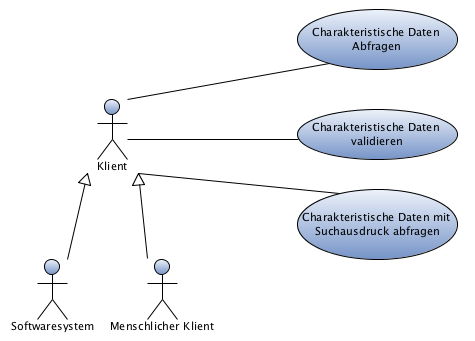
\includegraphics[width=0.75\textwidth]{images/usecases_plib.png}
	\caption{Use Case Übersicht}
	\label{fig:usecaseuebersicht}
\end{figure}

\subsection{Akteure}
Bei der Implementierung geht es um eine generische Schnittstelle. In den nachfolgenden Anwendungsfällen wird vom Akteur \enquote{Klient} gesprochen. Der Klient ist allgemein ein Nutzer der Schnittstelle, sei es als menschlicher Akteur welcher über eine Bedienerinterface die Schnittstelle benutzt oder eine direkte Maschinennutzung.    

%TODO Use Case Diagram

\subsection{Use Case Beschreibungen}

\subsubsection{Alle Charakteristische Daten eines Produkts abfragen}

{\small

\begin{description}
     \item[use case] Charakteristische Daten abfragen
     \item[  actors]~\\
     Klient
     \item[  precondition]~\\
     Der Klient verwendet einen gültigen Identifier.
     \item[  main flow]~\\
     Der Klient gibt einen Identifier (IRDI\footnote{International Registration Data Identifier}) einer Klasse von Elementen ein und sendet eine Anfrage ab. Die Anfrage wird auf Gültigkeit überprüft. Als Antwort bekommt er ein oder mehrere Datensätze von Elementen \footnote{Item, ISO 29002-10 Kapitel 5.3.2} mit den entsprechenden charakteristischen Daten \footnote{property\_values, ISO 29002-10 Kapitel 5.2.4}  des Elementes mit dem übergebenen Identifier zurück.
     \item[  postcondition]~\\
     Alle Daten aller Elemente der gewählten Klassen des Identifiers wurden zurückgegeben.    
     \item[  alternative flow] Properties auswählen ~\\
     Zusammen mit dem Identifier übergibt der Klient einen oder mehrere Property-Identifier und sendet diese erweiterte Anfrage ab.    
     \item[  postcondition]~\\
     Die mittels Property-Identifier ausgewählten Daten aller Elemente der gewählten Klassen wurden zurückgegeben.    
     \item[end] Charakteristische Daten abfragen
\end{description}

~\\

} %end small

\paragraph{Beispiel}

Ein Schraubendreher könnte folgendermaßen in einer Produktdatenbank repräsentiert werden:

\begin{description}\label{lab:schraubendreher}
\item[Klassen-Identifier] 0173-1\#01-AAA352\#4 
\item[Länge] 300mm
\item[Typ] Kreuz
\item[Spannungsfest] ja
\end{description}

Korrekterweise müssten anstatt der Attribute wie Länge oder Typ ebenfalls ein Identifier stehen. Die Benamungen sind hier zur besseren Lesbarkeit aufgelöst. 

Um nun alle Eigenschaften (Properties), wie Länge, Typ und Spannungsfest zu erhalten muss folgende Abfrage gesendet werden: 
\textbf{"Gib mir alle Items und alle Properties der Klasse mit dem Identifier 0173-1\#01-AAA352\#4 (Schraubendreher)".}
Das Ergebnis ist ein Item mit allen Attributen (Properties) der gewünschten Klassen und gegebenenfalls vorhandenen Unterklassen. In unserem Falle genau die oben angegebenen Werte.

Die XML-Abfrage sieht wie folgt aus:

\begin{lstlisting}[caption=Query Beispiel - Daten abfragen, language=XML, label=UseCaseDatenabfragen]
<?xml version="1.0" encoding="UTF-8"?>
<qy:query xsi:schemaLocation="...query query.xsd" xmlns:xsi="http://www.w3.org/2001/XMLSchema-instance" xmlns:cat="...catalogue" xmlns:val="...value" xmlns:qy="...query" xmlns:bas="...basic">
	<qy:class_ref>0173-1#01-AAA352#4</qy:class_ref>
</qy:query>
\end{lstlisting}

Eine Abfrage, welche die Properties der Klasse auswählt die zurückgeliefert werden sollen könnte lauten: 
\textbf{"Gib mir alle Items und die Properties Länge und Typ der Klasse mit dem Identifier 0173-1\#01-AAA352\#4 (Schraubendreher)".}
Das Ergebnis ist ein Item mit den gewünschten Attributen (Properties). 

Die XML-Abfrage:
\begin{lstlisting}[caption=Query Beispiel - Daten abfragen mit Propertyeinschränkung, language=XML, label=lst:UseCaseDatenabfragenProperty]

<?xml version="1.0" encoding="UTF-8"?>
<qy:query xsi:schemaLocation="...query query.xsd" xmlns:xsi="http://www.w3.org/2001/XMLSchema-instance" xmlns:cat="...catalogue" xmlns:val="...value" xmlns:qy="...query" xmlns:bas="...basic">
	<qy:class_ref>0173-1#01-AAA352#4</qy:class_ref>
	
	<!-- typ und laenge -->
	<qy:property_ref>0173-1#01-BBB111#1 0173-1#01-BBB222#1</qy:property_ref> 
	
</qy:query>
\end{lstlisting}

Listing \ref{lst:UseCaseDatenabfragenProperty} beinhaltet ein XML-Attribut property\_ref. Das wird mit gewünschten Property Identifier gefüllt, welche mit Leerzeichen getrennt werden. 

\subsubsection{Charakteristische Daten eines Produkts validieren}

{\small

\begin{description}
     \item[use case] Charakteristische Daten validieren
     \item[  actors]~\\
     Klient
     \item[  precondition]~\\
     Der Klient verwendet einen gültigen Identifier sowie auf den Identifier passende Daten..
     \item[  main flow]~\\
     Der Klient gibt einen Identifier eines Elementes (Klasse) ein. Zusätzlich übermittelt er zu diesem bekanntem Element Eigenschaften dieser Instanz des Elements und sendet eine Anfrage ab. Die Anfrage wird auf Gültigkeit überprüft. Als Antwort bekommt er ein oder mehrere Datensätze von Elementen mit den entsprechenden charakteristischen Daten zurück, auf welche die übergebenen Eigenschaften am besten zutreffen. 
     \item[  postcondition]~\\
     Alle Daten aller Elemente der gewählten Klassen des Identifiers werden zurückgegeben. Dies ermöglicht dem Klienten eine Validierung der ihm bereits bekannten Daten über ein Element. 
     \item[end] Charakteristische Daten validieren
\end{description}

~\\

} %end small

\paragraph{Beispiel}

In diesem Anwendungsfall verfügen wir bereits über Elemente/Wertenpaare einer bestimmten Klasse, z.B. eben jenen Schraubendreher

\textbf{"Ich habe hier ein mir bekanntes Item mit bestimmten Eigenschaften (Properties), Länge=300mm. Gib mir alle Items und alle Properties der Klasse mit dem Identifier 0173-1\#01-AAA352\#4 (Kreuzschraube) welche die mitgelieferten Eigenschaften haben".}
Das Ergebnis sind Items mit allen Properties der angegebenen Klasse, welche über die übergebenen Eigenschaften (Properties) verfügen. In unserem Fall vervollständigen wir unsere Properties mit den weiteren Properties "Typ" und "Spannungsfest".

Die XML-Abfrage sieht so aus:

\begin{lstlisting}[caption=Query Beispiel - Daten abfragen, language=XML, label=UseCaseDatenabfragen]
<?xml version="1.0" encoding="UTF-8"?>
<qy:query xsi:schemaLocation="...query query.xsd" xmlns:xsi="http://www.w3.org/2001/XMLSchema-instance" xmlns:cat="...catalogue" xmlns:val="...value" xmlns:qy="...query" xmlns:bas="...basic">
	<cat:item class_ref="0173-1#01-AAA352#4..">
		<cat:property_value property_ref="0173-1#01-BBB111#1">
			<val:integer_value></val:integer_value>
		</cat:property_value>
	</cat:item>
</qy:query>
\end{lstlisting}

\subsubsection{Chrarakteristische Daten mittels Suchausdruck abfragen }

{\small

\begin{description}
     \item[use case] Charakteristische Daten mit Suchausdruck abfragen
     \item[  actors]~\\
     Klient
     \item[  precondition]~\\
     Der Klient verwendet einen gültigen Identifier.
     \item[  main flow]~\\
     Der Klient gibt einen Identifier eines Elementes (Klasse) ein. Ferner übergibt er ein oder mehrere bekannte Property Identifier sowie passend dazu Werte zur Sucheinschränkung. 
     \item[  postcondition]~\\
     Alle Elemente auf jene diese Einschränkung der übergebenen Werte zutrifft wurden zurückgegeben. 
     \item[end] Charakteristische Daten mit Suchausdruck abfragen
\end{description}

~\\

} %end small

\paragraph{Beispiel}

Wir nehmen das Schraubendreher Beispiel aus \ref{lab:schraubendreher} zur Hand, und möchten eine Abfrage absenden, welche von der Klasse Schraubendreher alle Items erhalten soll die eine Länge zwischen 200 und 300 mm haben. 

Um nun alle Eigenschaften (Properties), wie Länge, Typ und Spannungsfest zu erhalten muss folgende Abfrage gesendet werden: 
\textbf{"Gib mir alle Items und alle Properties der Klasse mit dem Identifier 0173-1\#01-AAA352\#4 (Kreuzschraube)".}
Das Ergebnis ist ein Item mit allen Attributen (Properties) der gewünschten Klassen und gegebenenfalls vorhandenen Unterklassen. In unserem Falle genau die oben angegebenen Werte.

Die XML-Abfrage sieht so aus:

\begin{lstlisting}[caption=Query Beispiel - Daten abfragen, language=XML, label=UseCaseDatenabfragen]
<?xml version="1.0" encoding="UTF-8"?>
<qy:query xsi:schemaLocation="...query query.xsd" xmlns:xsi="http://www.w3.org/2001/XMLSchema-instance" xmlns:cat="...catalogue" xmlns:val="...value" xmlns:qy="...query" xmlns:bas="...basic">
	<qy:class_ref>0173-1#01-AAA352#4</qy:class_ref>
	<qy:characteristic_data_query_expression>
		<qy:range>
			<qy:property_reference property_ref="0173-1#01-BBB111#1"/>
			<qy:min_value>200</qy:min_value>
			<qy:max_value>300</qy:max_value>
			<qy:is_inclusive>true</qy:is_inclusive>
		</qy:range>
	</qy:characteristic_data_query_expression>
</qy:query>
\end{lstlisting}


%\section{Automatisierte Benutzerebene}
%Der Unterschied zur manuellen Benutzerebene ist der, dass hierbei automatisiert Daten angefragt und übermittelt werden. Es findet keine Mensch zu %Maschine Kommunikation statt sondern eine Maschine zu Maschine Kommunikation. 
%Ziel der automatisierten Anfragen ist das Abgleichen oder Validieren von Massendaten eines (Teil)-Katalogs. 

%\begin{description}
%\item[Alle Klassen abfragen] Der Klient sendet eine Anfrage und erhält alle vorhandene Klassen (ohne Items).
%\item[Items einer Klasse abgleichen] Der Klient möchte seine Daten abgleichen und fragt alle Items einer Klasse ab.  
%\item[Items einer Klasse validieren] Der Klient möchte seine Daten validieren und fragt alle Items einer Klasse ab.
%\end{description}

% Index
\renewcommand{\indexname}{Index}
\addcontentsline{toc}{chapter}{Index}
\printindex

\end{document}

